\documentclass[review]{elsarticle}

\usepackage{multirow}
\usepackage{lineno}
\usepackage{xspace}
\usepackage{threeparttable}
\usepackage{subfig}
\modulolinenumbers[5]

%% Journal name here
\journal{Journal Title}

%% `Elsevier LaTeX' style
\bibliographystyle{elsarticle-num}
%%%%%%%%%%%%%%%%%%%%%%%

%%%% packages and definitions (optional)
\usepackage{placeins}
\usepackage{booktabs} % nice rules (thick lines) for tables
\usepackage{microtype} % improves typography for PDF
\usepackage{hhline}
\usepackage{amsmath}
\usepackage{subfig}

\usepackage{threeparttable, tablefootnote}

\usepackage{tabularx}
\usepackage{siunitx}

%% Special typesetting for Cyclus
\newcommand{\Cyclus}{\textsc{Cyclus}\xspace}%
\newcommand{\Cycamore}{\textsc{Cycamore}\xspace}%
\graphicspath{{images/}}

% tikz %
\usepackage{tikz}
\usetikzlibrary{positioning, arrows, decorations, shapes}

\usetikzlibrary{shapes.geometric,arrows}
\tikzstyle{process} = [rectangle, rounded corners, minimum width=3cm, minimum height=1cm,text centered, draw=black, fill=blue!30]
\tikzstyle{object} = [ellipse, rounded corners, minimum width=3cm, minimum height=1cm,text centered, draw=black, fill=green!30]
\tikzstyle{arrow} = [thick,->,>=stealth]

% hyperref %
\usepackage[hidelinks]{hyperref}
% after hyperref %
\usepackage{cleveref}
\usepackage{datatool}
\usepackage[acronym,toc]{glossaries}
\include{acros}

\makeglossaries

\begin{document}
\begin{frontmatter}
\title{Coupled Neutronics/Thermal-Hydraulics Analysis of the Molten Salt
Fast Reactor}

%\date{}                     % uncomment if you don't need date to appear

% Authors
\author[uiuc]{Sun Myung Park}
\author[uiuc]{Kathryn D. Huff\corref{corrauthor}}
%% If unsure, google "corresponding author" for more info
\cortext[corrauthor]{Corresponding Author}
\ead{kdhuff@illinois.edu}


% Institutes of the authors
\input{institutions}

\begin{keyword}
molten salt reactor \sep
molten salt fast reactor \sep
multiphysics \sep
safety analysis \sep 
reactor dynamics \sep
high performance computing
\end{keyword}

\input{abstract}
\end{frontmatter}
\glsresetall

%% Shows line numbers
\linenumbers

\section{Introduction}

The \gls{MSR} concept is one of the six advanced nuclear reactor concepts
shortlisted by the \gls{GIF} for improved safety, sustainability, efficiency
and cost over the current generations of reactors
\cite{gif_technology_2002} \cite{gif_technology_2014}. This has led
to growing
research interest in \glspl{MSR} in the past two decades, after a relative
lull that followed shortly after the shutdown of the first and only fully
operational \gls{MSR} reactors, the \gls{ARE} and \gls{MSRE}, back in the
1950s and 1960s \cite{haubenreich_msre_1964}
\cite{haubenreich_experience_1970}. In particular, \glspl{MSR} concepts boast
significant advantages in reactor safety and sustainability arising from the
liquid fuel form \cite{elsheikh_safety_2013}. The thermal expansion of the
fuel contributes significantly to the
strongly negative temperature reactivity coefficients observed in most
\gls{MSR} designs. In the event of a power excursion and the accompanying
temperature rise, this reactivity feedback is quite prompt and limits the
maximum temperature that the reactor may reach during this type of accident
scenario. Using liquid fuel also allows for continuous online reprocessing
which impacts sustainability in two main ways: increasing overall fuel burnup
through the continuous removal of parasitic fission products and minimal
downtime, and improving breeding ratios in the context of the thorium fuel
cycle where the intermediate Pa is temporarily removed from the reactor core
to prevent the undesirable formation of U234.

However, this new feature also brought about novel computational
challenges in simulating the transient behavior of \glspl{MSR}; the
neutronics and thermal-hydraulics are more tightly coupled due to the strong
temperature reactivity coefficient, and the additional advection coupling
terms. Furthermore, we have to account for the movement of \glspl{DNP} as
they are now generated directly within the primary coolant loop. Therefore,
the choice of coupling methods for each set of physics requires careful
consideration. Existing reactor system-level codes and modeling approaches
for conventional \glspl{LWR} analysis contain simplifying assumptions in
multiphysics coupling and other areas that render the techniques unsuitable
for simulating \gls{MSR}. Thus, making minor modifications to these codes
without changing the underlying algorithms is not the best approach for
\gls{MSR} safety analysis.

In the past two decades, researchers have developed several
new tools for simulating steady-state and transient behavior in \glspl{MSR}.
Many of the earlier efforts featured simplifications in simulating
thermal-hydraulics by solving 1-D Navier-Stokes equations or using
predetermined uniform velocity fields \cite{krepel_dyn3d-msr_2007}
\cite{kophazi_development_2009}. In more recent years, there has been
significant progress towards fully coupled, spatial codes that feature
2-D axisymmetric or full 3-D models. In 2011, Cammi et al.
\cite{cammi_multi-physics_2011} performed an ``\gls{MPM}'' analysis
of a simplified 2-D axisymmetric model of a single MSBR fuel channel using
the commercial finite-element analysis software COMSOL Multiphysics. The
physics were implemented through the two-group neutron diffusion
equations, and the \gls{RANS} standard $k-\epsilon$ turbulence model, for the
neutronics and thermal-hydraulics respectively. The
authors emphasized the need for proper full coupling of the multiphysics, and
presented both steady-state and transient results in various
scenarios such as reactivity insertions, changes in pumping rate, and the
presence of periodic perturbations. This approach featured again in a later
paper by Fiorina et al. \cite{fiorina_modelling_2014} in 2014 for a 2-D
axisymmetric model of the
\gls{MSFR}. The authors presented results from the Politecnico di Milano
COMSOL-based approach, and another approach by researchers from Delft
University of Technology, where they coupled their in-house neutronics and
thermal-hydraulics codes, DALTON and HEAT respectively. With multi-group
neutron diffusion and \gls{RANS} formulations on ultra-fine meshes, both
models showed good agreement in the steady-state neutron flux, temperature,
and \gls{DNP} distributions, and in the power responses following various
accident transient initiations. Aufiero et al. \cite{aufiero_development_2014}
concurrently developed
a full-core 3-D model of the \gls{MSFR} on OpenFOAM, albeit with one-group
neutron diffusion to reduce computational load. With the 3-D model, the
authors could simulate the asymmetric reactor response to the failure of a
single pump in the sixteen-pump \gls{MSFR} configuration. The authors also
provided some quantitative data supporting the use of implicit coupling over
explicit coupling to obtain accurate solutions of the transient cases.
Recognizing the huge computational burden required for full 3-D simulations, 
later authors came up with innovative ways to alleviate this issue such as
selective geometrical reduced order modeling for various components of a
reactor based on the importance of the physical phenomena being simulated
\cite{zanetti_geometric_2015}, or using a novel, efficient method for
neutronics calculations \cite{laureau_transient_2017}.

In this paper, we present steady-state and transient analysis of the
\gls{MSFR} concept using Moltres \cite{lindsay_introduction_2018}, a
multiphysics finite element analysis tool
for simulating \glspl{MSR}. Similar to the COMSOL and OpenFOAM, Moltres
solves the deterministic multi-group neutron diffusion and thermal-hydraulics
\glspl{PDE} simultaneously on the same mesh. It supports up to 3-D meshes and
scales well for an arbitrary number of processors. As a code under active
development, the main objective of this paper is to benchmark Moltres' current
capabilities against similar codes in the context of the reference
\gls{MSFR} concept. A previous study \cite{lindsay_introduction_2018}
showcasing Moltres' capabilities with
the \gls{MSRE} design had shown good agreement with legacy
\gls{MSRE} data and strong parallel performance with up to 768 processors.
We leverage on this powerful feature to provide high fidelity \gls{MSFR}
simulation results at reasonable wall-clock times.

The paper is organized as follows. (Insert paper format)

\section{Molten Salt Fast Reactor}

The \gls{MSFR} is a reference design of a circulating-fuel \gls{MSR} developed
under the EURATOM \gls{EVOL} \cite{euratom_final_2015} and \gls{SAMOFAR}
\cite{kloosterman_20_2017} projects. The core of the
\gls{MSFR} consists of a 9 m$^3$ pool of fuel salt flowing upwards
\cite{serp_molten_2014}. At the top
of the core, the fuel salt flow separates into sixteen individual peripheral
loops, passing through the pumps, heat exchangers, and other instrumentation,
before flowing back into the active core region from the bottom. The core is
surrounded axially by nickel alloy reflectors, and radially by a toroidal
blanket tank containing fertile salt for
breeding. A layer of boron carbide absorber further protects the outer
components from excessive neutron damage. The main reactor specifications and
schematic view are shown in Table \ref{table:msfr} and Fig. \ref{fig:msfr}
respectively. 
%
\begin{table}[htb!]
	\caption{Main specifications of the \gls{MSFR} concept
				\cite{serp_molten_2014}.}
	\centering
	\begin{tabular}{ l r }
		\hline
		Parameter & Value \\
		\hline
		Thermal/Electric output [MW$_{\text{th}}$/MW$_{\text{e}}$] & 3000 /
		1500 
		\\
		Salt volume [m$^3$] & 18 \\
		Salt fraction in core & 0.5 \\
		Number of circulation loops & 16 \\
		Nominal flow rate [kg s$^{-1}$] & 18500  \\
		Nominal circulation time [s] & 4.0 \\
		Inlet/outlet temperature [K] & 923 / 1023 \\
		Blanket volume [m$^3$] & 7.3\\
		\hline
	\end{tabular}
	\label{table:msfr}
\end{table}
%
\begin{figure}[htb!] 
	\centering
	\includegraphics[width=0.6\textwidth]{MSFR}
	\caption{Schematic view of the MSFR concept \cite{serp_molten_2014}.}
	\label{fig:msfr}
\end{figure}

For the $^{232}$Th/$^{233}$U breeder configuration, the fuel and blanket salts
are composed of eutectic mixtures of 77.5\% LiF - 22.5\% AcF$_4$, where
AcF$_4$ represents actinide fluorides, uranium and thorium fluoride
\cite{serp_molten_2014}. A mole
fraction of approximately 1\% $^{233}$U is required for criticality; most
studies adjust the composition to achieve criticality at a uniform temperature
973 K as was done in the \gls{MSFR} neutronics benchmark paper
\cite{brovchenko_neutronic_2019}. Breeding ratios of up to 1.1 are expected
for the \gls{MSFR} \cite{fiorina_molten_2013}.

According to the design specifications, the inlet and outlet temperatures of
the fuel salt are to be 923 K and 1023 K respectively. This was motivated by
the desire for a 50 K minimum buffer between the operating temperatures
and the melting point of the salt \cite{euratom_final_2015}.
Having a secondary coolant loop adds a layer of containment between the
radioactive material and the outside environment. The exact specifications of
the heat exchanger and the secondary coolant loop are yet to be determined.
Thus, we assumed a secondary coolant temperature of 823 K with a heat transfer
coefficient value that corresponds to the intended 100 K temperature drop in
the fuel salt.

\section{Methodology}

This section discusses the modeling approach and the codes used in this paper.

\subsection{Geometry}

For this work, we used the reference square-cylindrical \gls{MSFR} design to
benchmark Moltres against results published by Fiorina et al. and Aufiero et
al. It is a 2-D axisymmetric design with the sixteen individual external loops
homogenized into a single outer loop as shown in figure *. This is the geometry
used in this work to calculate the multi-group cross sections and various
group constants for each material region in Serpent 2. 

\subsection{Subsection}

\begin{figure}[h]
        \centering
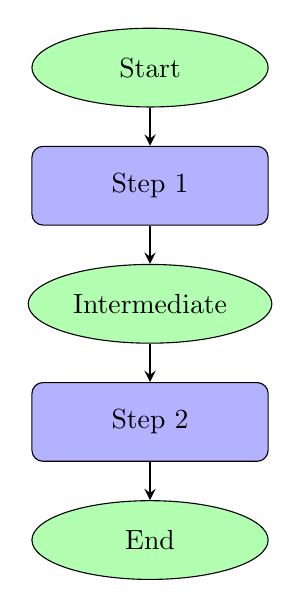
\begin{tikzpicture}[node distance=1.5cm]
\node (start) [object] {Start};
\node (step1) [process, below of=start] {Step 1};
\node (intermediate) [object, below of=step1] {Intermediate};
\node (step2) [process, below of=intermediate] {Step 2};
\node (end) [object, below of=step2]{End};

\draw [arrow] (start) -- (step1); 
\draw [arrow] (step1) -- (intermediate);
\draw [arrow] (intermediate) -- (step2); 
\draw [arrow] (step2) -- (end);
\end{tikzpicture}
\caption{A caption for the flowchart.}
\label{fig:comp}
\end{figure}

\input{results}
\section{Conclusion}
This is the conclusion section.

Reprocessing schemes also require intensive research because
of the various constraints pertaining to maintaining reactor criticality,
operational safety, and favorable salt redox conditions while maximizing
breeding ratios.

\input{acks}

\bibliography{bibliography.bib}

% Prof. Huff discourages appendices in journal articles.
% But, if you must, include one like so:
%\pagebreak
%\input{appendix}

\end{document}
